%% Session 05 – Neural Network: Feedforward and Backpropagation
%% Deep Learning Course, IIIT Dharwad
%% Generated from lecture transcript and visual extractions

\documentclass[12pt,a4paper]{article}
\usepackage{amsmath,amsthm,amssymb,mathtools}
\usepackage{tikz}
\usetikzlibrary{arrows.meta,positioning,shapes.geometric,calc,fit,backgrounds}
\usepackage{graphicx}
\usepackage{booktabs,tabularx,multirow}
\usepackage[ruled,vlined,linesnumbered]{algorithm2e}
\usepackage[most]{tcolorbox}
\usepackage{hyperref}
\usepackage[capitalize,noabbrev]{cleveref}
\usepackage[margin=1in]{geometry}
\usepackage{fancyhdr}
\usepackage{enumitem}
\usepackage{xcolor}

%% ── tcolorbox environments ──────────────────────────────────────────────────
\newtcolorbox{keyinsight}[1][]{colback=blue!5!white,colframe=blue!75!black,
  fonttitle=\bfseries,title=Key Insight,#1}
\newtcolorbox{example}[1][]{colback=green!5!white,colframe=green!75!black,
  fonttitle=\bfseries,title=Example,#1}
\newtcolorbox{warningbox}[1][]{colback=red!5!white,colframe=red!75!black,
  fonttitle=\bfseries,title=Warning,#1}

%% ── amsthm environments ─────────────────────────────────────────────────────
\newtheorem{theorem}{Theorem}[section]
\newtheorem{lemma}[theorem]{Lemma}
\newtheorem{definition}{Definition}[section]
\newtheorem{remark}{Remark}[section]

%% ── Page style ───────────────────────────────────────────────────────────────
\pagestyle{fancy}
\fancyhf{}
\rhead{Deep Learning -- Session 05}
\lhead{IIIT Dharwad}
\cfoot{\thepage}
\renewcommand{\headrulewidth}{0.4pt}

%% ── Misc macros ──────────────────────────────────────────────────────────────
\newcommand{\R}{\mathbb{R}}
\newcommand{\Loss}{\mathcal{L}}
\newcommand{\wh}[1]{w^{h}_{#1}}
\newcommand{\yhat}{\hat{y}}

\hypersetup{
  colorlinks=true,
  linkcolor=blue!60!black,
  urlcolor=blue!60!black,
  pdftitle={Session 05: Neural Network Feedforward and Backpropagation},
}

% ─────────────────────────────────────────────────────────────────────────────
\begin{document}

% ════════════════════════════════════════════════════════════════════════════
%  TITLE PAGE
% ════════════════════════════════════════════════════════════════════════════
\begin{titlepage}
  \centering
  \vspace*{2cm}

  {\LARGE\bfseries Deep Learning Course\\[0.4em]
   \rule{\linewidth}{0.5pt}\\[0.6em]
   Session 05: Neural Network\\Feedforward and Backpropagation\\
   \rule{\linewidth}{0.5pt}}

  \vspace{1.5cm}

  \begin{tcolorbox}[colback=blue!5!white,colframe=blue!50!black,width=0.85\linewidth]
    \centering
    \begin{tabular}{ll}
      \textbf{Session Number:} & 05 \\[4pt]
      \textbf{Topic:}          & Multi-layer feedforward networks, differentiable \\
                               & activation functions, backpropagation, chain rule \\[4pt]
      \textbf{Deck:}           & \texttt{03-DL-NeuralNetworkIntroduction} \\[4pt]
      \textbf{Instructors:}    & Prof.\ S~R~M~Prasanna \& Dr.\ Sunil Saumya \\[4pt]
      \textbf{Institution:}    & Dept.\ of Data Science \& Artificial Intelligence \\
                               & Indian Institute of Information Technology Dharwad \\[4pt]
      \textbf{Duration:}       & 1 hour 51 minutes 36 seconds \\[4pt]
      \textbf{Video:}          & \url{https://vimeo.com/1142296251} \\
    \end{tabular}
  \end{tcolorbox}

  \vspace{1.5cm}

  \begin{abstract}
    \noindent
    Session~05 extends the single-layer perceptron framework to
    \emph{multi-layer feedforward neural networks} (MLFFNNs).  The session
    opens with a recap of why linearly non-separable problems require hidden
    layers, then identifies the \emph{hard learning problem}: the perceptron
    learning rule cannot be applied to hidden-layer weights because no target
    output is available there.  The resolution is replacing the
    non-differentiable step function with \emph{differentiable sigmoidal
    activations} (logistic and hyperbolic tangent), enabling the
    \emph{backpropagation algorithm} (generalised delta rule) to propagate
    error gradients from the output layer back through every hidden layer via
    the chain rule.  A complete numerical forward pass on an IQ/CGPA
    prediction example (ReLU hidden activations, linear output) is worked
    through, followed by the derivation of the first backpropagation
    gradients $\partial\Loss/\partial v_1$, $\partial\Loss/\partial v_2$, and
    $\partial\Loss/\partial b_3$.
  \end{abstract}

  \vfill
  {\small Notes compiled from lecture transcript and slide visual extractions.\\
   Reference textbook: B.~Yegnanarayana, \emph{Artificial Neural Networks},
   PHI, New Delhi, 1999.}
\end{titlepage}

% ════════════════════════════════════════════════════════════════════════════
%  TABLE OF CONTENTS
% ════════════════════════════════════════════════════════════════════════════
\tableofcontents
\newpage

% ════════════════════════════════════════════════════════════════════════════
%  1. INTRODUCTION
% ════════════════════════════════════════════════════════════════════════════
\section{Introduction}
\label{sec:intro}

The single-layer perceptron, equipped with a step (hard-limiting) output
function, can learn any \emph{linearly separable} classification boundary.
However, a vast class of real-world problems---from XOR-type logical functions
to complex regression tasks---requires non-linear decision surfaces.
Session~04 established that adding more layers of perceptrons can, in
principle, represent arbitrary convex (two layers) or non-convex (three
layers) decision regions.  Session~05 confronts the natural follow-up
question: \emph{how do we train such a multi-layer network?}

The answer unfolds in two conceptual steps.
\begin{enumerate}[label=\textbf{Step \arabic*.},leftmargin=3em]
  \item \textbf{Identify the obstacle.}  In a multi-layer network only the
    output-layer activations are directly observable; the hidden-layer target
    outputs are \emph{unknown}.  Without a target, the simple
    error $= \text{target} - \text{actual}$ cannot be formed at hidden nodes,
    so the perceptron learning rule breaks down.  Prof.~Prasanna terms this
    the \emph{hard learning problem}.

  \item \textbf{Resolve it with differentiable activations and the chain
    rule.}  Replacing the step function with smooth sigmoidal functions
    (logistic or hyperbolic tangent) makes every output differentiable.  This
    allows the output-layer error to be \emph{propagated backwards} layer by
    layer through the chain rule---the celebrated
    \emph{backpropagation algorithm}, also known as the
    \emph{generalised delta rule}.
\end{enumerate}

The session then walks through a concrete numerical example: a two-input
(IQ, CGPA) network with one hidden layer of two ReLU neurons and a linear
output neuron predicting a student's salary package.

\begin{keyinsight}[title=Session~05 in One Sentence]
  Backpropagation solves the hard learning problem by using differentiable
  activation functions and the chain rule to express hidden-layer errors in
  terms of the observable output-layer error, enabling gradient descent over
  \emph{all} network weights simultaneously.
\end{keyinsight}

% ════════════════════════════════════════════════════════════════════════════
%  2. BACKGROUND AND PREREQUISITES
% ════════════════════════════════════════════════════════════════════════════
\section{Background and Prerequisites}
\label{sec:background}

\subsection{The Perceptron and its Limitations}
\label{subsec:perceptron}

A single perceptron computes a weighted sum of its inputs followed by a
hard-limiting (step) output function.  For an input vector
$\mathbf{a} = (a_1, \ldots, a_I)^{\top}$ and weight vector $\mathbf{w}$, the
perceptron output is
\begin{equation}
  s = \operatorname{sgn}\!\left(\mathbf{w}^{\top}\mathbf{a} - \theta\right),
  \qquad \operatorname{sgn}(x) =
  \begin{cases} +1 & x \geq 0, \\ -1 & x < 0. \end{cases}
  \label{eq:perceptron}
\end{equation}
The \emph{perceptron learning rule} updates weights as
\begin{equation}
  \Delta \mathbf{w} = \eta\,\delta\,\mathbf{a},
  \qquad \delta = b - \operatorname{sgn}(\mathbf{w}^{\top}\mathbf{a}),
  \label{eq:percep-learning}
\end{equation}
where $b$ is the desired (target) output and $\eta > 0$ is the learning rate.
This rule requires a \emph{known target} at every neuron; a requirement
impossible to satisfy for hidden layers.

\subsection{Representing Nonlinear Decision Regions}
\label{subsec:nonlinear}

\begin{definition}[Convex and Non-convex Problems]
  \label{def:convex}
  A classification problem is \emph{convex} if the decision region of every
  class is a convex set.  It is \emph{non-convex} otherwise.
\end{definition}

The architectural depth required scales with the complexity of the desired
boundary:
\begin{itemize}
  \item \textbf{Linearly separable:} 1 layer (input + output perceptron).
  \item \textbf{Convex non-linear:} 2 layers (input + 1 hidden + output).
  \item \textbf{Non-convex:} 3 layers (input + 2 hidden + output).
\end{itemize}

While this representational hierarchy was understood, \emph{training} these
deeper networks remained an open problem for nearly a decade---the neural
network field stalled until the backpropagation algorithm provided a
practical solution.

\subsection{Supervised Learning Setup}
\label{subsec:supervised}

Throughout this session the learning task is \emph{supervised}: given a
dataset $\{(\mathbf{a}(m), \mathbf{b}(m))\}_{m=1}^{M}$ of input--output
pairs, the goal is to find weights such that for each pattern $m$ the network
output $\mathbf{b}'(m)$ approximates the desired output $\mathbf{b}(m)$ with
small error.  The squared error for pattern $m$ is
\begin{equation}
  E(m) = \frac{1}{2}\sum_{k=1}^{K}\bigl[b_k(m) - b'_k(m)\bigr]^2,
  \label{eq:error}
\end{equation}
where $K$ is the number of output units.  The factor of $\tfrac{1}{2}$ is
conventional and simplifies later derivatives.

% ════════════════════════════════════════════════════════════════════════════
%  3. THREE-LAYER FEEDFORWARD NETWORK
% ════════════════════════════════════════════════════════════════════════════
\section{The Three-Layer Feedforward Neural Network}
\label{sec:architecture}

\subsection{Network Notation (Figure 4.12)}
\label{subsec:notation}

Following Yegnanarayana (1999), the canonical three-layer network (called a
\emph{two-layer perceptron} in that text because the linear input layer is not
counted as a ``learning'' layer) has the following structure.

\begin{definition}[Three-Layer MLFFNN]
  \label{def:threelayer}
  A three-layer multi-layer feedforward neural network (MLFFNN) consists of:
  \begin{itemize}
    \item \textbf{Input layer}: $I$ linear units indexed by $i = 1,\ldots,I$,
      with activations $a_i$.
    \item \textbf{Hidden layer}: $J$ nonlinear units indexed by $j = 1,\ldots,J$,
      with outputs $s_j^h$.
    \item \textbf{Output layer}: $K$ nonlinear units indexed by $k = 1,\ldots,K$,
      with outputs $s_k^o$.
  \end{itemize}
  Weights from input unit $i$ to hidden unit $j$ are denoted $w_{ji}^h$.
  Weights from hidden unit $j$ to output unit $k$ are denoted $w_{kj}$.
\end{definition}

The superscript $h$ on input-to-hidden weights is purely notational---it
distinguishes the two sets of weights and is dropped for the hidden-to-output
set.

\subsection{TikZ Diagram: Three-Layer FFNN Architecture}
\label{subsec:arch-tikz}

\cref{fig:threelayer} shows the fully-connected three-layer architecture.

\begin{figure}[htbp]
\centering
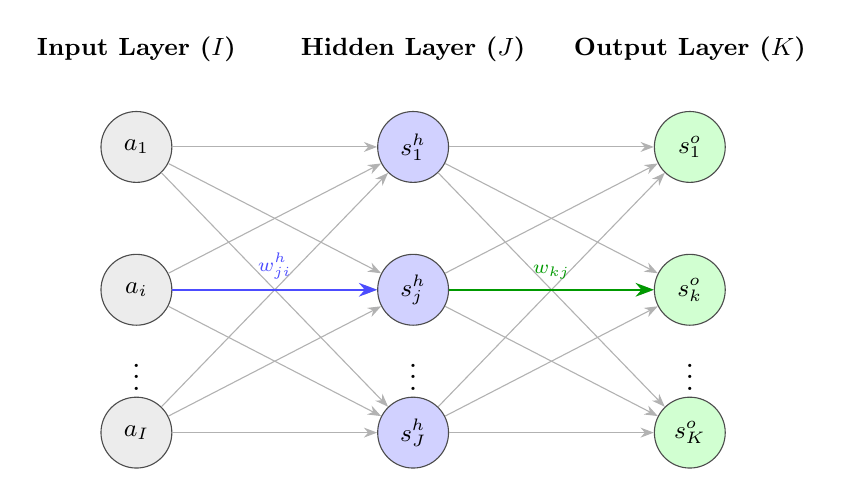
\begin{tikzpicture}[
    node distance=1.6cm and 2.6cm,
    neuron/.style={circle, draw=black!70, fill=white, minimum size=0.9cm,
                   font=\small},
    inputn/.style={neuron, fill=gray!15},
    hiddenn/.style={neuron, fill=blue!18},
    outputn/.style={neuron, fill=green!18},
    bias/.style={rectangle, draw=black!50, fill=yellow!20, minimum size=0.7cm,
                 font=\scriptsize},
    >=Stealth
  ]

  %% Input layer
  \node[inputn] (i1) {$a_1$};
  \node[inputn, below=0.9cm of i1] (i2) {$a_i$};
  \node[inputn, below=0.9cm of i2] (i3) {$a_I$};

  %% Hidden layer
  \node[hiddenn, right=2.6cm of i1] (h1) {$s_1^h$};
  \node[hiddenn, below=0.9cm of h1] (h2) {$s_j^h$};
  \node[hiddenn, below=0.9cm of h2] (h3) {$s_J^h$};

  %% Output layer
  \node[outputn, right=2.6cm of h1] (o1) {$s_1^o$};
  \node[outputn, below=0.9cm of o1] (o2) {$s_k^o$};
  \node[outputn, below=0.9cm of o2] (o3) {$s_K^o$};

  %% Input → Hidden (selected edges)
  \foreach \src in {i1,i2,i3}{
    \foreach \dst in {h1,h2,h3}{
      \draw[->, gray!60, thin] (\src) -- (\dst);
    }
  }

  %% Annotate one weight
  \draw[->, blue!70, thick] (i2) -- node[above, sloped, font=\scriptsize]
        {$w_{ji}^h$} (h2);

  %% Hidden → Output (selected edges)
  \foreach \src in {h1,h2,h3}{
    \foreach \dst in {o1,o2,o3}{
      \draw[->, gray!60, thin] (\src) -- (\dst);
    }
  }

  %% Annotate one weight
  \draw[->, green!60!black, thick] (h2) -- node[above, sloped, font=\scriptsize]
        {$w_{kj}$} (o2);

  %% Layer labels
  \node[above=0.5cm of i1, font=\bfseries\small] {Input Layer ($I$)};
  \node[above=0.5cm of h1, font=\bfseries\small] {Hidden Layer ($J$)};
  \node[above=0.5cm of o1, font=\bfseries\small] {Output Layer ($K$)};

  %% Vertical dots
  \node[font=\large] at ($(i2)!0.5!(i3) + (0,-0.1cm)$) {$\vdots$};
  \node[font=\large] at ($(h2)!0.5!(h3) + (0,-0.1cm)$) {$\vdots$};
  \node[font=\large] at ($(o2)!0.5!(o3) + (0,-0.1cm)$) {$\vdots$};

\end{tikzpicture}
\caption{Three-layer multi-layer feedforward neural network (Figure~4.12 from
  Yegnanarayana, 1999).  The input layer is linear; the hidden and output
  layers are nonlinear.  Every input unit connects to every hidden unit
  (weights $w_{ji}^h$), and every hidden unit connects to every output unit
  (weights $w_{kj}$).}
\label{fig:threelayer}
\end{figure}

\subsection{Forward Propagation Equations}
\label{subsec:forward-eqs}

The computation for each layer proceeds as a two-step process: a linear
\emph{weighted summation} followed by a nonlinear \emph{activation function}.

\paragraph{Hidden layer.}
For hidden unit $j$:
\begin{align}
  x_j^h &= \sum_{i=1}^{I} w_{ji}^h\, a_i + b_j^h,
  \label{eq:hidden-net} \\
  s_j^h &= f\!\left(x_j^h\right),
  \label{eq:hidden-act}
\end{align}
where $b_j^h$ is the bias of hidden unit $j$ and $f(\cdot)$ is the
differentiable activation function.

\paragraph{Output layer.}
For output unit $k$:
\begin{align}
  x_k^o &= \sum_{j=1}^{J} w_{kj}\, s_j^h + b_k^o,
  \label{eq:output-net} \\
  s_k^o &= f\!\left(x_k^o\right).
  \label{eq:output-act}
\end{align}

\begin{keyinsight}[title=Why ``Feedforward''?]
  Information flows strictly from left (input) to right (output): input
  activations $\to$ hidden layer $\to$ output layer.  There are no feedback
  connections during inference.  The name \emph{feedforward} reflects this
  unidirectional signal flow.
\end{keyinsight}

% ════════════════════════════════════════════════════════════════════════════
%  4. DIFFERENTIABLE ACTIVATION FUNCTIONS
% ════════════════════════════════════════════════════════════════════════════
\section{Differentiable Activation Functions}
\label{sec:activations}

\subsection{Why Differentiability Matters}
\label{subsec:why-diff}

The step function used in the classical perceptron is:
\begin{equation}
  f_{\mathrm{step}}(x) = \begin{cases} 1 & x \geq 0, \\ 0 & x < 0. \end{cases}
  \label{eq:step}
\end{equation}
Its derivative is zero everywhere except at $x=0$, where it is undefined.
This means that $\partial E / \partial w_{ji}^h$ involves $f'(x_j^h) = 0$
for all $x_j^h \neq 0$, killing any gradient signal that would adjust hidden
weights.  The backpropagation algorithm requires \emph{non-zero} derivatives
throughout.

\begin{warningbox}[title=The Step Function Cannot be Used in Hidden Layers]
  If $f$ is the step function, then $f'(x) = 0$ almost everywhere.  The
  gradient $\partial E / \partial w_{ji}^h$ evaluates to zero regardless of
  the error, making it \emph{impossible} to update input-to-hidden weights via
  gradient descent.  This is the root cause of the ``hard learning problem''.
\end{warningbox}

\subsection{The Logistic (Sigmoid) Function}
\label{subsec:logistic}

The logistic function with slope parameter $\beta > 0$ is:
\begin{equation}
  f(x) = \frac{1}{1 + \exp(-2\beta x)},
  \qquad f(x) \in (0, 1).
  \label{eq:logistic}
\end{equation}
Its derivative has a convenient closed form:
\begin{equation}
  \dot{f}(x) = 2\beta\, f(x)\bigl(1 - f(x)\bigr).
  \label{eq:logistic-deriv}
\end{equation}
Key values: $f(0) = 0.5$; $f(x) \to 1$ as $x \to +\infty$; $f(x) \to 0$
as $x \to -\infty$.

\begin{remark}
  The standard logistic sigmoid $\sigma(x) = (1+e^{-x})^{-1}$ is a special
  case of \cref{eq:logistic} with $\beta = \tfrac{1}{2}$, giving
  $\dot{\sigma}(x) = \sigma(x)(1-\sigma(x))$.
\end{remark}

\subsection{The Hyperbolic Tangent Function}
\label{subsec:tanh}

The hyperbolic tangent activation is:
\begin{equation}
  f(x) = \tanh(\beta x) = \frac{e^{\beta x} - e^{-\beta x}}{e^{\beta x} + e^{-\beta x}},
  \qquad f(x) \in (-1, 1).
  \label{eq:tanh}
\end{equation}
Its derivative is:
\begin{equation}
  \dot{f}(x) = \beta\bigl(1 - f^2(x)\bigr).
  \label{eq:tanh-deriv}
\end{equation}
The symmetric range $(-1,+1)$ often leads to faster convergence than logistic
because the mean activation is centred at zero, reducing the covariate shift
between layers.

\subsection{The ReLU Function}
\label{subsec:relu}

Modern deep networks frequently use the Rectified Linear Unit (ReLU):
\begin{equation}
  f(x) = \max(0, x),
  \qquad \dot{f}(x) = \begin{cases} 1 & x > 0, \\ 0 & x \leq 0. \end{cases}
  \label{eq:relu}
\end{equation}
ReLU does not saturate for positive inputs (unlike sigmoid/tanh), avoiding
the vanishing gradient problem in deeper architectures.  In this session's
numerical example, ReLU is used in the hidden layer while the output layer
uses a \emph{linear} (identity) activation for regression.

\subsection{Comparison Table}
\label{subsec:activation-table}

\cref{tab:activations} summarises the four activation functions encountered in
this session.

\begin{table}[htbp]
\centering
\caption{Summary of activation functions.  $\beta$ is a slope parameter
  (default $\beta = 0.5$ for logistic and tanh).}
\label{tab:activations}
\renewcommand{\arraystretch}{1.4}
\begin{tabularx}{\linewidth}{lXXXX}
\toprule
\textbf{Function} & \textbf{Formula} & \textbf{Derivative} & \textbf{Range}
  & \textbf{Typical Use} \\
\midrule
Step (hard limiting)
  & $\mathbf{1}[x \geq 0]$
  & $0$ (a.e.)
  & $\{0,1\}$
  & Output of classical perceptron only \\
Logistic (sigmoid)
  & $\frac{1}{1+e^{-2\beta x}}$
  & $2\beta f(1-f)$
  & $(0,1)$
  & Hidden/output layers (binary classification) \\
Tanh
  & $\tanh(\beta x)$
  & $\beta(1-f^2)$
  & $(-1,1)$
  & Hidden layers (zero-centred) \\
ReLU
  & $\max(0,x)$
  & $\mathbf{1}[x>0]$
  & $[0,\infty)$
  & Hidden layers in deep networks \\
\bottomrule
\end{tabularx}
\end{table}

% ════════════════════════════════════════════════════════════════════════════
%  5. BACKPROPAGATION: THE GENERALISED DELTA RULE
% ════════════════════════════════════════════════════════════════════════════
\section{Backpropagation: The Generalised Delta Rule}
\label{sec:backprop}

\subsection{Gradient Descent on the Error Surface}
\label{subsec:grad-descent}

Backpropagation is a \emph{gradient descent} algorithm.  The error $E(m)$
defined in \cref{eq:error} is a surface in the space of all weights.  The
goal is to find the weight configuration that corresponds to a (local) minimum
of this surface.  Moving in the direction of steepest descent requires
computing the gradient $\nabla_{\mathbf{w}} E$.

The weight update rule for any weight $w_{ij}$ is:
\begin{equation}
  \Delta w_{ij} = -\eta\,\frac{\partial E(m)}{\partial w_{ij}},
  \qquad \eta > 0,
  \label{eq:grad-descent}
\end{equation}
\begin{equation}
  w_{ij}(m+1) = w_{ij}(m) + \Delta w_{ij}.
  \label{eq:weight-update}
\end{equation}
The negative sign ensures movement \emph{downhill} on the error surface.

\subsection{The Hard Learning Problem Revisited}
\label{subsec:hard-learning}

For output-layer weights $w_{kj}$, computing $\partial E / \partial w_{kj}$
is straightforward because the error $E(m)$ depends directly on the
output-layer activations $s_k^o$.  For hidden-layer weights $w_{ji}^h$,
however, $E(m)$ depends on $w_{ji}^h$ only \emph{indirectly}, through
$s_j^h \to s_k^o$.  The chain rule bridges this gap.

\begin{keyinsight}[title=The Core Idea of Backpropagation]
  Even though no target is available at hidden units, the error computed at
  the output layer can be \emph{mathematically expressed} in terms of
  hidden-layer outputs, provided those outputs are produced by a differentiable
  activation function.  The chain rule then gives a closed-form gradient for
  every weight in the network.
\end{keyinsight}

\subsection{Deriving the Output-Layer Gradient}
\label{subsec:output-gradient}

For output unit $k$ with net input $x_k^o = \sum_j w_{kj} s_j^h + b_k^o$:
\begin{align}
  \frac{\partial E}{\partial w_{kj}}
    &= \frac{\partial E}{\partial s_k^o}
       \cdot\frac{\partial s_k^o}{\partial x_k^o}
       \cdot\frac{\partial x_k^o}{\partial w_{kj}} \notag \\[4pt]
    &= \bigl[-(b_k - s_k^o)\bigr]
       \cdot \dot{f}(x_k^o)
       \cdot s_j^h.
  \label{eq:output-grad}
\end{align}
Defining the \emph{output delta}:
\begin{equation}
  \delta_k^o = (b_k - s_k^o)\,\dot{f}(x_k^o),
  \label{eq:delta-output}
\end{equation}
the update becomes $\Delta w_{kj} = \eta\,\delta_k^o\,s_j^h$.

\subsection{Deriving the Hidden-Layer Gradient}
\label{subsec:hidden-gradient}

For hidden unit $j$ with net input $x_j^h = \sum_i w_{ji}^h\,a_i + b_j^h$:
\begin{align}
  \frac{\partial E}{\partial w_{ji}^h}
    &= \sum_{k=1}^{K}
       \frac{\partial E}{\partial s_k^o}
       \cdot\frac{\partial s_k^o}{\partial x_k^o}
       \cdot\frac{\partial x_k^o}{\partial s_j^h}
       \cdot\frac{\partial s_j^h}{\partial x_j^h}
       \cdot\frac{\partial x_j^h}{\partial w_{ji}^h} \notag \\[4pt]
    &= \dot{f}(x_j^h)
       \left[\sum_{k=1}^{K} \delta_k^o\,w_{kj}\right]
       \cdot a_i.
  \label{eq:hidden-grad}
\end{align}
Defining the \emph{hidden delta} as:
\begin{equation}
  \delta_j^h = \dot{f}(x_j^h)\sum_{k=1}^{K}\delta_k^o\,w_{kj},
  \label{eq:delta-hidden}
\end{equation}
the update rule for hidden-layer weights is $\Delta w_{ji}^h = \eta\,\delta_j^h\,a_i$.

\begin{remark}
  The hidden delta $\delta_j^h$ in \cref{eq:delta-hidden} is a weighted sum of
  \emph{output deltas} $\delta_k^o$, propagated back through the weights
  $w_{kj}$ and modulated by the local derivative $\dot{f}(x_j^h)$.  This is
  why the algorithm is called \emph{back}propagation: the error signal travels
  from output to input.
\end{remark}

\subsection{Comparison: Discrete vs.\ Continuous Delta Rule}
\label{subsec:discrete-vs-continuous}

\cref{tab:delta-rules} contrasts the classical (discrete) perceptron learning
law with the generalised (continuous/differentiable) delta rule.

\begin{table}[htbp]
\centering
\caption{Discrete perceptron learning law vs.\ generalised delta rule.}
\label{tab:delta-rules}
\renewcommand{\arraystretch}{1.5}
\begin{tabularx}{\linewidth}{lXX}
\toprule
\textbf{Property} & \textbf{Discrete (Perceptron)} & \textbf{Generalised Delta Rule} \\
\midrule
Output function $f$
  & Step / signum (non-differentiable)
  & Sigmoid, tanh, ReLU (differentiable) \\
Weight update rule
  & $\Delta w = \eta\,(b - \operatorname{sgn}(\mathbf{w}^{\top}\mathbf{a}))\,\mathbf{a}$
  & $\Delta w_{ij} = -\eta\,\partial E/\partial w_{ij}$ \\
Applicable to
  & Output layer only (target known)
  & All layers (chain rule handles hidden layers) \\
Error definition
  & Direct: $\delta = b - s$
  & Gradient: $\partial E / \partial w$ via chain rule \\
Key innovation
  & $\delta$ proportional to error $b - s$
  & $\delta$ proportional to error \emph{times} $\dot{f}(x)$ \\
Convergence
  & Guaranteed (linearly separable data)
  & Convergence to local minimum (not guaranteed globally) \\
\bottomrule
\end{tabularx}
\end{table}

% ════════════════════════════════════════════════════════════════════════════
%  6. THE TRAINING LOOP
% ════════════════════════════════════════════════════════════════════════════
\section{The Neural Network Training Loop}
\label{sec:training-loop}

\subsection{Forward and Backward Passes}
\label{subsec:fwd-bwd}

Training a neural network alternates between two phases in every iteration
(epoch/mini-batch):

\begin{enumerate}[label=\textbf{Phase \arabic*.}]
  \item \textbf{Forward Pass.} Feed the input through the network
    layer-by-layer to obtain the prediction $\yhat$.
  \item \textbf{Loss Computation.} Compute the scalar loss
    $\Loss(\yhat, y)$.
  \item \textbf{Backward Pass.} Use the chain rule to compute
    $\partial\Loss/\partial w$ for every weight $w$ in the network.
  \item \textbf{Parameter Update.} Update all weights using the gradient
    descent rule of \cref{eq:weight-update}.
\end{enumerate}

\cref{fig:training-loop} illustrates this iterative cycle.

\begin{figure}[htbp]
\centering
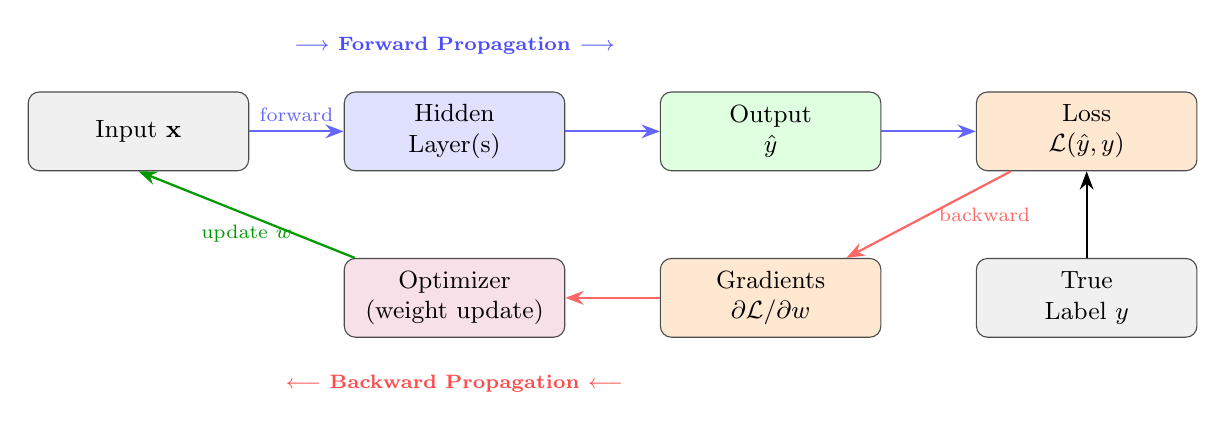
\begin{tikzpicture}[
    box/.style={rectangle, draw=black!70, rounded corners=4pt,
                minimum width=2.8cm, minimum height=1.0cm,
                align=center, font=\small, fill=white},
    inputbox/.style={box, fill=gray!12},
    hidbox/.style={box, fill=blue!12},
    outbox/.style={box, fill=green!12},
    lossbox/.style={box, fill=orange!18},
    optbox/.style={box, fill=purple!12},
    >=Stealth,
    node distance=1.2cm and 0.8cm
  ]

  %% Forward pass nodes (top row, left to right)
  \node[inputbox] (input) {Input $\mathbf{x}$};
  \node[hidbox, right=1.2cm of input] (hidden1) {Hidden\\Layer(s)};
  \node[outbox, right=1.2cm of hidden1] (output) {Output\\$\yhat$};
  \node[lossbox, right=1.2cm of output] (loss) {Loss\\$\Loss(\yhat, y)$};

  %% True label node
  \node[inputbox, below=1.1cm of loss] (true) {True\\Label $y$};

  %% Optimizer node
  \node[optbox, below=1.1cm of hidden1] (optim) {Optimizer\\(weight update)};

  %% Gradient node
  \node[lossbox, below=1.1cm of output] (grads) {Gradients\\$\partial\Loss/\partial w$};

  %% Forward arrows
  \draw[->, thick, blue!60] (input) -- node[above, font=\scriptsize]{forward} (hidden1);
  \draw[->, thick, blue!60] (hidden1) -- (output);
  \draw[->, thick, blue!60] (output) -- (loss);
  \draw[->, thick] (true) -- (loss);

  %% Backward arrows
  \draw[->, thick, red!60] (loss) -- node[right, font=\scriptsize]{backward} (grads);
  \draw[->, thick, red!60] (grads) -- (optim);
  \draw[->, thick, green!60!black] (optim) --
        node[below, font=\scriptsize]{update $w$} (input.south);

  %% Labels
  \node[above=0.35cm of hidden1, font=\bfseries\scriptsize, blue!70]
        {$\longrightarrow$ Forward Propagation $\longrightarrow$};
  \node[below=0.35cm of optim, font=\bfseries\scriptsize, red!70]
        {$\longleftarrow$ Backward Propagation $\longleftarrow$};

\end{tikzpicture}
\caption{The neural network training loop.  In every iteration the forward
  pass computes predictions, the loss is evaluated, gradients are
  back-propagated, and the optimizer updates all weights.  This cycle repeats
  until the loss is minimised.}
\label{fig:training-loop}
\end{figure}

\subsection{Backpropagation Algorithm}
\label{subsec:bp-algo}

\cref{alg:backprop} gives the complete single-pattern backpropagation
procedure for a three-layer network.

\begin{algorithm}[htbp]
\DontPrintSemicolon
\caption{Backpropagation for a Three-Layer MLFFNN (single pattern)}
\label{alg:backprop}
\KwIn{Input $\mathbf{a}$, desired output $\mathbf{b}$, learning rate $\eta$,
      weights $\{w_{ji}^h\}$ and $\{w_{kj}\}$, biases $\{b_j^h\}$ and $\{b_k^o\}$}
\KwOut{Updated weights and biases}
\BlankLine
\tcp{--- Forward Pass ---}
\For{$j = 1$ \KwTo $J$}{
  $x_j^h \leftarrow \sum_{i} w_{ji}^h\,a_i + b_j^h$\;
  $s_j^h \leftarrow f(x_j^h)$\;
}
\For{$k = 1$ \KwTo $K$}{
  $x_k^o \leftarrow \sum_{j} w_{kj}\,s_j^h + b_k^o$\;
  $s_k^o \leftarrow f(x_k^o)$\;
}
\BlankLine
\tcp{--- Compute Loss ---}
$E \leftarrow \frac{1}{2}\sum_{k}(b_k - s_k^o)^2$\;
\BlankLine
\tcp{--- Backward Pass: Output Layer Deltas ---}
\For{$k = 1$ \KwTo $K$}{
  $\delta_k^o \leftarrow (b_k - s_k^o)\,\dot{f}(x_k^o)$\;
}
\BlankLine
\tcp{--- Backward Pass: Hidden Layer Deltas ---}
\For{$j = 1$ \KwTo $J$}{
  $\delta_j^h \leftarrow \dot{f}(x_j^h)\,\sum_{k} \delta_k^o\,w_{kj}$\;
}
\BlankLine
\tcp{--- Weight Updates ---}
\For{$k = 1$ \KwTo $K$}{
  \For{$j = 1$ \KwTo $J$}{
    $w_{kj} \leftarrow w_{kj} + \eta\,\delta_k^o\,s_j^h$\;
  }
  $b_k^o \leftarrow b_k^o + \eta\,\delta_k^o$\;
}
\For{$j = 1$ \KwTo $J$}{
  \For{$i = 1$ \KwTo $I$}{
    $w_{ji}^h \leftarrow w_{ji}^h + \eta\,\delta_j^h\,a_i$\;
  }
  $b_j^h \leftarrow b_j^h + \eta\,\delta_j^h$\;
}
\Return{Updated weights and biases}\;
\end{algorithm}

\begin{keyinsight}[title=Computational Complexity]
  Each forward pass requires $O(I \cdot J + J \cdot K)$ multiplications.
  The backward pass has the same order of complexity.  Training thus scales
  linearly in the number of parameters---a key reason backpropagation is
  computationally feasible even for large networks.
\end{keyinsight}

% ════════════════════════════════════════════════════════════════════════════
%  7. NUMERICAL EXAMPLE
% ════════════════════════════════════════════════════════════════════════════
\section{Numerical Example: IQ/CGPA to Salary Prediction}
\label{sec:example}

Dr.~Sunil Saumya walks through a concrete one-iteration example.
The problem is a regression task: predict a student's salary package (LPA)
from their IQ score and CGPA.

\subsection{Network Architecture}
\label{subsec:example-arch}

The network has:
\begin{itemize}
  \item Two real-valued inputs: $x_1 = \text{IQ}$ and $x_2 = \text{CGPA}$.
  \item One hidden layer with two neurons ($h_1$, $h_2$), each using
    \textbf{ReLU} activation.
  \item One output neuron ($\yhat$) using \textbf{linear} (identity) activation.
  \item Bias nodes: $b_1 = b_2 = b_3 = 1$.
\end{itemize}

\subsection{Weights and Data}
\label{subsec:example-weights}

The initial weights are:
\begin{align}
  w_{11} &= 0.02, & w_{12} &= 0.50, \notag \\
  w_{21} &= 0.04, & w_{22} &= -0.30, \notag \\
  v_1    &= 1.20, & v_2    &= 0.80.
  \label{eq:init-weights}
\end{align}
The first training data point is:
\begin{equation}
  x_1 = 80 \;\text{(IQ)}, \quad x_2 = 8 \;\text{(CGPA)}, \quad y = 3 \;\text{(LPA)}.
  \label{eq:data-point}
\end{equation}

\subsection{Forward Pass}
\label{subsec:forward-pass}

\paragraph{Hidden neuron $h_1$.}
\begin{align}
  z_1 &= w_{11}x_1 + w_{12}x_2 + b_1 \notag \\
      &= 0.02 \times 80 + 0.50 \times 8 + 1 \notag \\
      &= 1.60 + 4.00 + 1.00 = 6.60, \\
  h_1 &= \mathrm{ReLU}(z_1) = \max(0,\;6.60) = \mathbf{6.60}.
  \label{eq:h1}
\end{align}

\paragraph{Hidden neuron $h_2$.}
\begin{align}
  z_2 &= w_{21}x_1 + w_{22}x_2 + b_2 \notag \\
      &= 0.04 \times 80 + (-0.30) \times 8 + 1 \notag \\
      &= 3.20 - 2.40 + 1.00 = 1.80, \\
  h_2 &= \mathrm{ReLU}(z_2) = \max(0,\;1.80) = \mathbf{1.80}.
  \label{eq:h2}
\end{align}

\paragraph{Output neuron (linear activation).}
\begin{align}
  \yhat &= v_1 h_1 + v_2 h_2 + b_3 \notag \\
        &= 1.20 \times 6.60 + 0.80 \times 1.80 + 1 \notag \\
        &= 7.92 + 1.44 + 1.00 = \mathbf{10.36}.
  \label{eq:yhat}
\end{align}

\begin{example}[title=Forward Pass Summary]
  \begin{center}
  \renewcommand{\arraystretch}{1.3}
  \begin{tabular}{lll}
    \toprule
    \textbf{Quantity} & \textbf{Value} & \textbf{Remark} \\
    \midrule
    $z_1 = w_{11}x_1 + w_{12}x_2 + b_1$ & $6.60$ & Pre-activation, $h_1$ \\
    $h_1 = \mathrm{ReLU}(z_1)$           & $6.60$ & Positive, so passes through \\
    $z_2 = w_{21}x_1 + w_{22}x_2 + b_2$ & $1.80$ & Pre-activation, $h_2$ \\
    $h_2 = \mathrm{ReLU}(z_2)$           & $1.80$ & Positive, so passes through \\
    $\yhat = v_1h_1 + v_2h_2 + b_3$      & $10.36$ & Network prediction \\
    $y$                                   & $3.00$  & True label \\
    $\Loss = (y - \yhat)^2$               & $54.15$ & Very high; weights need updating \\
    \bottomrule
  \end{tabular}
  \end{center}
\end{example}

\subsection{Loss Computation}
\label{subsec:loss}

Using squared-error loss:
\begin{align}
  \Loss &= (y - \yhat)^2 = (3 - 10.36)^2 = (-7.36)^2 = 54.17.
  \label{eq:loss-val}
\end{align}

The loss of $54.17$ is very large (the best possible is $0$), indicating that
the randomly initialised weights are far from optimal.  Backpropagation will
now compute how each weight contributed to this loss and update them
accordingly.

\subsection{Backward Pass: Output-Layer Gradients}
\label{subsec:backward-pass}

The loss function and its derivative with respect to $\yhat$ are:
\begin{align}
  \Loss &= (y - \yhat)^2, \\
  \frac{\partial \Loss}{\partial \yhat} &= 2(\yhat - y) = 2(10.36 - 3) = 14.72.
  \label{eq:dloss-dyhat}
\end{align}

Since $\yhat = v_1 h_1 + v_2 h_2 + b_3$, the partial derivatives are:

\paragraph{Gradient with respect to $v_1$.}
\begin{equation}
  \frac{\partial \Loss}{\partial v_1}
    = \frac{\partial \Loss}{\partial \yhat} \cdot \frac{\partial \yhat}{\partial v_1}
    = 2(\yhat - y) \cdot h_1
    = 14.72 \times 6.60 = \mathbf{97.15}.
  \label{eq:grad-v1}
\end{equation}

\paragraph{Gradient with respect to $v_2$.}
\begin{equation}
  \frac{\partial \Loss}{\partial v_2}
    = \frac{\partial \Loss}{\partial \yhat} \cdot \frac{\partial \yhat}{\partial v_2}
    = 2(\yhat - y) \cdot h_2
    = 14.72 \times 1.80 = \mathbf{26.50}.
  \label{eq:grad-v2}
\end{equation}

\paragraph{Gradient with respect to $b_3$.}
\begin{equation}
  \frac{\partial \Loss}{\partial b_3}
    = \frac{\partial \Loss}{\partial \yhat} \cdot \frac{\partial \yhat}{\partial b_3}
    = 2(\yhat - y) \cdot 1
    = \mathbf{14.72}.
  \label{eq:grad-b3}
\end{equation}

\begin{keyinsight}[title=Chain Rule is the Engine of Backpropagation]
  Each gradient is computed by chaining partial derivatives along the path
  from the weight to the loss.  For $v_1$: the path is
  $v_1 \to \yhat \to \Loss$, giving
  $\partial\Loss/\partial v_1
   = (\partial\Loss/\partial\yhat)\cdot(\partial\yhat/\partial v_1)
   = 2(\yhat-y)\cdot h_1$.
  The same pattern extends to weights in earlier layers by continuing the
  chain backward.
\end{keyinsight}

\subsection{Weight Update (one iteration)}
\label{subsec:weight-update-example}

Using learning rate $\eta = 0.01$, the updated output-layer weights after one
step of gradient descent are:
\begin{align}
  v_1^{\mathrm{new}} &= v_1 - \eta\,\frac{\partial\Loss}{\partial v_1}
                      = 1.20 - 0.01 \times 97.15 = 1.20 - 0.97 = \mathbf{0.23}, \\
  v_2^{\mathrm{new}} &= v_2 - \eta\,\frac{\partial\Loss}{\partial v_2}
                      = 0.80 - 0.01 \times 26.50 = 0.80 - 0.27 = \mathbf{0.53}, \\
  b_3^{\mathrm{new}} &= b_3 - \eta\,\frac{\partial\Loss}{\partial b_3}
                      = 1.00 - 0.01 \times 14.72 = 1.00 - 0.15 = \mathbf{0.85}.
  \label{eq:weight-updates-example}
\end{align}
These updated weights would then be used in the next forward pass, which
should produce a prediction closer to the true value $y = 3$.

\subsection{Extending the Chain Rule to Hidden-Layer Weights}
\label{subsec:chain-rule-hidden}

To update hidden-layer weight $w_{11}$ (from input $x_1$ to $h_1$), the
chain rule must be extended one step further:
\begin{equation}
  \frac{\partial\Loss}{\partial w_{11}}
    = \frac{\partial\Loss}{\partial\yhat}
      \cdot\frac{\partial\yhat}{\partial h_1}
      \cdot\frac{\partial h_1}{\partial z_1}
      \cdot\frac{\partial z_1}{\partial w_{11}}.
  \label{eq:chain-hidden}
\end{equation}
Evaluating each factor:
\begin{align}
  \frac{\partial\Loss}{\partial\yhat}   &= 2(\yhat - y) = 14.72, \\
  \frac{\partial\yhat}{\partial h_1}    &= v_1 = 1.20, \\
  \frac{\partial h_1}{\partial z_1}     &= \mathrm{ReLU}'(z_1) = 1 \quad (z_1 = 6.60 > 0), \\
  \frac{\partial z_1}{\partial w_{11}}  &= x_1 = 80.
  \label{eq:chain-factors}
\end{align}
Therefore:
\begin{equation}
  \frac{\partial\Loss}{\partial w_{11}}
    = 14.72 \times 1.20 \times 1 \times 80 = \mathbf{1412.9}.
  \label{eq:grad-w11}
\end{equation}

\begin{example}[title=Computation Graph for $\partial\Loss/\partial w_{11}$]
  The dependency chain is:
  \[
    w_{11}
    \;\xrightarrow{\times x_1}\; z_1
    \;\xrightarrow{\mathrm{ReLU}}\; h_1
    \;\xrightarrow{\times v_1}\; \yhat
    \;\xrightarrow{(y-\yhat)^2}\; \Loss.
  \]
  Each arrow contributes one factor to the chain rule product.
\end{example}

% ════════════════════════════════════════════════════════════════════════════
%  8. SIGNIFICANCE AND CONTEXT
% ════════════════════════════════════════════════════════════════════════════
\section{Historical Significance and Modern Context}
\label{sec:context}

\subsection{The ``Hard Learning Problem'' and the Decade of Silence}
\label{subsec:history}

As Prof.~Prasanna explains in the lecture, the existence of multi-layer
perceptron \emph{architectures} was known well before a training algorithm
existed.  Researchers understood that:
\begin{itemize}
  \item A three-layer network can represent any convex decision region.
  \item A four-layer network can represent any non-convex decision region
    (universal approximation).
\end{itemize}
Yet training such networks was impossible with the perceptron learning rule
because the hidden-layer target outputs are unknown.  This ``hard learning
problem'' caused the neural network field to stagnate for nearly a decade.

The backpropagation algorithm---attributable to Rumelhart, Hinton, and
Williams (1986), though independently discovered earlier by others---resolved
the impasse by the single insight: \emph{replace the non-differentiable step
function with a smooth sigmoid, then apply the chain rule}.

\subsection{Connection to Modern Deep Learning}
\label{subsec:modern}

The backpropagation principle remains the backbone of all modern deep learning:
\begin{itemize}
  \item Large language models with 96--100+ transformer layers use the same
    fundamental forward/backward loop.
  \item Automatic differentiation libraries (PyTorch, JAX, TensorFlow) build
    \emph{computation graphs} at runtime and apply backpropagation
    automatically.
  \item ReLU, introduced as an empirical improvement over sigmoid, resolves the
    \emph{vanishing gradient problem} that afflicts sigmoid/tanh in very deep
    networks.
\end{itemize}

\begin{keyinsight}[title=Backpropagation Today]
  While modern architectures (transformers, graph neural networks, diffusion
  models) are far more complex than the three-layer MLFFNN, they all compute
  gradients via the same chain rule that Dr.~Prasanna derives in this session.
  Understanding backpropagation at this level is foundational to understanding
  any deep learning system.
\end{keyinsight}

% ════════════════════════════════════════════════════════════════════════════
%  9. SUMMARY AND CONCLUSION
% ════════════════════════════════════════════════════════════════════════════
\section{Summary and Conclusion}
\label{sec:summary}

Session~05 covered the theoretical and practical foundations of training a
multi-layer feedforward neural network.  The key ideas are summarised below.

\subsection*{Main Contributions of the Session}

\begin{enumerate}[label=\textbf{\arabic*.}]
  \item \textbf{Multi-layer architecture.}  A three-layer MLFFNN (input +
    hidden + output) can represent non-convex decision boundaries and general
    continuous functions, overcoming the representational limit of the
    single-layer perceptron.

  \item \textbf{The hard learning problem.}  The perceptron learning rule
    requires a target output at every neuron.  Hidden layers have no external
    target, making direct application of the delta rule impossible.

  \item \textbf{Differentiable activations.}  Replacing the step function with
    logistic/tanh/ReLU functions provides everywhere non-zero derivatives,
    enabling gradient information to flow backward through the network.

  \item \textbf{Backpropagation (generalised delta rule).}  The chain rule
    allows the output-layer error to be decomposed layer by layer.  The
    resulting weight update rule $\Delta w = -\eta\,\partial E/\partial w$
    applies uniformly to every weight in the network.

  \item \textbf{Numerical forward pass.}  For the IQ/CGPA example with
    $x_1=80$, $x_2=8$, $y=3$: the network predicts $\yhat = 10.36$ giving
    squared error $\Loss = 54.17$.

  \item \textbf{First backpropagation gradients.}  The output-layer gradients
    $\partial\Loss/\partial v_1 = 97.15$, $\partial\Loss/\partial v_2 = 26.50$,
    and $\partial\Loss/\partial b_3 = 14.72$ were derived using the chain rule,
    initiating the backward pass.
\end{enumerate}

\subsection*{Key Equations}

\begin{align}
  E(m)              &= \tfrac{1}{2}\sum_k [b_k - s_k^o]^2
                     \tag{Error} \\
  \Delta w_{ij}     &= -\eta\,\frac{\partial E}{\partial w_{ij}}
                     \tag{Gradient Descent} \\
  \delta_k^o        &= (b_k - s_k^o)\,\dot{f}(x_k^o)
                     \tag{Output Delta} \\
  \delta_j^h        &= \dot{f}(x_j^h)\sum_k \delta_k^o w_{kj}
                     \tag{Hidden Delta} \\
  w \leftarrow w    &+ \eta\,\delta\,(\text{incoming activation})
                     \tag{Weight Update}
\end{align}

\subsection*{Looking Ahead}

The session ends with the chain-rule derivation of output-layer gradients.
Subsequent sessions will:
\begin{itemize}
  \item Derive the full backpropagation pass for hidden-layer weights
    $w_{ji}^h$.
  \item Demonstrate the complete one-iteration update on the
    IQ/CGPA example.
  \item Implement backpropagation in PyTorch, verifying the manually
    computed gradients.
\end{itemize}

\vspace{1em}
\begin{tcolorbox}[colback=gray!5!white, colframe=gray!50!black,
                  title={\bfseries Session~05 -- Quick Reference Card}]
\begin{tabular}{ll}
\textbf{Algorithm} & Backpropagation (generalised delta rule) \\
\textbf{Network}   & 3-layer MLFFNN: input $I$, hidden $J$, output $K$ \\
\textbf{Activations} & Logistic, tanh (differentiable); ReLU (piecewise linear) \\
\textbf{Loss}      & $E = \tfrac{1}{2}\sum_k(b_k - s_k^o)^2$ \\
\textbf{Update}    & $w \leftarrow w - \eta\,\partial E/\partial w$ \\
\textbf{Key tool}  & Chain rule: $\partial E/\partial w = \prod (\partial/\partial)$ along path \\
\textbf{Example}   & $x_1=80, x_2=8 \Rightarrow \yhat=10.36$, loss $=54.17$ \\
\end{tabular}
\end{tcolorbox}

\end{document}
